The primary goal of this project was do develop the compiler backend. 
Initially little attention was paid to structuring larger projects composed of multiple source files and dependencies. While smaller applications can work fine with a single script of regular expressions, in the tasks on natural language processing its common to build large codebases composed of millions of linguistic rules. Being able to manage and organise them efficiently becomes a major issue. 

The compiler builds automata using our special version fo Glushkov's construction, which is capable of compiling subexpressions independently of each other. The results are returned in form of singly linked graph. This format allows one to parallelise compilation and split work across multiple files. For instance user could create two files \texttt{file1.mealy} and \texttt{file2.mealy}, define some variable in the first one and the use it in the second.
\begin{lstlisting}
file1.mealy:
    var1 = 'abc'
file2.mealy:
    var2 = ('prefix' var1 'suffix')*
\end{lstlisting}
Such a feature is not native to the compiler backend itself (it only parses continuous string of input) and has been delegated to the build system as an independent application instead. 

The easiest approach to implementing build system would be by concatenating all source files into one large steam of input and then feed it into the compiler.
For instance 
\begin{lstlisting}
concatenatedFiles.mealy:
    //from file1.mealy
    var1 = 'abc'
    //from file2.mealy
    var2 = ('prefix' var1 'suffix')*
\end{lstlisting}
It could be easily done with a simple Bash script or a couple of Makefiles. Despite being very straightforward, such a solution has multiple flaws. The order of concatenation matters a lot. The compiler requires that every variable is defined before being used. Should the order get mistakenly swapped, the compilation would fail. For instance 
\begin{lstlisting}
concatenatedFiles.mealy:
    //from file2.mealy
    var2 = ('prefix' var1 'suffix')* 
    // var1 used before definition!
    //from file1.mealy
    var1 = 'abc'
\end{lstlisting}
As a result, it would be user's obligation to ensure correct order of concatenation, which might quickly become unmaintainable in large projects. Second problem stems from linear types. The compiler follows the semantics of linear logic and a variable once consumed should not be reused. An explicit copy is always necessary. Hence the order of definition and usage of all variables is even more important than in other general-purpose languages that do not have linear types. For instance this will compile
\begin{lstlisting}
X = 'a'
Y = !!X 'b'
Z = X 'c'
\end{lstlisting}
but this one will fail
\begin{lstlisting}
X = 'a'
Z = X 'c'
Y = !!X 'b'
\end{lstlisting}
Third problem is that managing dependencies and building packages would become impossible. For example we might imagine code, which includes some library 
\begin{lstlisting}
include libX
X = f  // f is defined in libX
\end{lstlisting}
If in the future a new version of the library is released, it might happen that variable X is added and suddenly our code becomes invalid because we're trying to redefine X.

Our initial thought was to introduce a special function \texttt{import!('filepath')}, which would load any variable from a precompiled binary file. Then the user would write code as follows
\begin{lstlisting}
X = import!('lib/libX/f')
\end{lstlisting}
This approach suffers from one logistic problem. If user decided to split their code into several files and then import the necessary automata at will, the build system would need to detect the correct compilation order of all files. For instance if there were two files like these
\begin{lstlisting}
file X.mealy:
    a = 'a'
file Y.mealy:
    b = import!('X/a')
\end{lstlisting}
then the build system would need to first compile \texttt{X.mealy} and produce binary file \texttt{X} and only then compilation of \texttt{Y.mealy} would become possible. The major problem appears when cyclic dependencies between files arise
\begin{lstlisting}
file X.mealy:
    X = import!('Y/Y')
file Y.mealy:
    Y = import!('X/X')
\end{lstlisting}
While it's possible to create a built tool capable of detecting such problems and notifying the user, its main disadvantage is that in some cases, there might be cyclic dependency between files, despite not introducing cyclic dependencies between automata themselves. As a result, logically valid regular expressions would be prematurely rejected by build system. For example
\begin{lstlisting}
file X.mealy:
    X1 = import!('Y/Y1')
    X2 = 'a'
file Y.mealy:
    Y1 = 'b'
    Y2 = import!('X/X2')
\end{lstlisting}
The final solution we settled for was to split compilation into three phases. First the build system scans all files (in parallel) and builds abstract syntax trees of all variable definitions. In those trees there would be references to other variables that could be defined anywhere else in the project. Then in the second phase the variables would be scanned and a dependency graph would be built. We used a specialised data structure for efficiently working with directed acyclic graphs. If at any point a cycle was introduced, the build system would throw an error. Finally in the last phase every node in the graph would be compiled in parallel. For optimal performance, multiple threads would take vertices in topological order. If there is a directed edge from vertex $v_1$ to $v_2$ (meaning that variable $v_2$ depends on $v_1$), then $v_1$ will be added to the queue before $v_2$. Threads process queue entries in the FIFO order. 

In the first phase, the parser that scans source files has been reused from the compiler backend. More precisely, the grammar of syntax is taken from the library but the build system has its own implementation of \texttt{SolomonoffGrammarListener}. Parsing is then performed using the standard ANTLR functions
\begin{lstlisting}
SolomonoffGrammarLexer lexer =
  new SolomonoffGrammarLexer(sourceFile);
SolomonoffGrammarParser parser =
  new SolomonoffGrammarParser(new CommonTokenStream(lexer));

parser.addErrorListener(new BaseErrorListener() {
    public void syntaxError(Recognizer<?, ?> recognizer, 
            Object offendingSymbol, 
            int line,
            int charPositionInLine, 
            String msg, 
            RecognitionException e) {
         System.err.println("line " + line 
         + ":" + charPositionInLine 
         + " " + msg + " " + e);
    }
});

final SolomonoffWeightedParser listener =
  new SolomonoffWeightedParser(collector, sourceFile, compiler);
ParseTreeWalker.DEFAULT.walk(listener, parser.start());
\end{lstlisting}
The listener is responsible for building abstract syntax tree for each variable and storing all definitions. Here is a fragment of ANTLR grammar that forms the list of variable definitions 
\begin{lstlisting}
funcs :
    funcs exponential='!!'? ID '=' mealy_union  # FuncDef
    | 
;
\end{lstlisting} 
Whenever some definition is parsed, the following listener callback is invoked
\begin{lstlisting}
@Override
public void exitFuncDef(FuncDefContext funcDefContext) {
    String currentVariableID = funcDefContext.ID().getText();
    SolomonoffWeighted def = stack.pop();
    collector.define(currentVariable, def);
}
\end{lstlisting}
The integral part of listener is the \texttt{collector} object. It is responsible for storing all defined variables and remembering their respective abstract syntax trees. Initially, it was enough to store a \texttt{HashMap} within the \texttt{SolomonoffWeightedParser} object and register variables using 
\begin{lstlisting}
HashMap<String,SolomonoffWeighted> idToAST = 
    new HashMap<>();
    
@Override
public void exitFuncDef(FuncDefContext funcDefContext) {
    String currentVariableID = funcDefContext.ID().getText();
    SolomonoffWeighted def = stack.pop();
    idToAST.put(currentVariable, def);
}
\end{lstlisting}
Later it was changed to a more complicated implementation, which is
\begin{lstlisting}
ConcurrentHashMap<String,SolomonoffWeighted> idToAST;
SolomonoffWeightedParser(
    ConcurrentHashMap<String,SolomonoffWeighted> shared){
    this.idToAST = shared;
}
@Override
public void exitFuncDef(FuncDefContext funcDefContext) {
    String currentVariableID = funcDefContext.ID().getText();
    SolomonoffWeighted def = stack.pop();
    idToAST.put(currentVariable, def);
}
\end{lstlisting}
In such a way, it became possible to create multiple instances of 
\texttt{SolomonoffWeightedParser} and run all of them in parallel, while the results of parsing could still be collected into one joint map.
The use of \texttt{ConcurrentHashMap} instead of regular \texttt{HashMap} allows for concurrent insertions, without requiring any locks or synchronization. 

The abstract syntax tree closely follows the definition of Solomonoff's syntax. Its formal grammar is fairly simple and mimics the mathematical definition of regular expressions
\begin{lstlisting}
mealy_union
:
    (mealy_concat bar='|') * mealy_concat # MealyUnion
;

mealy_concat
:
    mealy_concat mealy_Kleene_closure
    | mealy_Kleene_closure # MealyEndConcat
;

mealy_Kleene_closure
:
    mealy_prod  (star='*' | plus='+' | optional='?') 
    | mealy_prod # MealyNoKleeneClosure
;

mealy_prod
:
    mealy_atomic colon=':' StringLiteral # MealyProduct
    | mealy_atomic colon=':' Codepoint # MealyProductCodepoints
    | mealy_atomic # MealyEpsilonProduct
;

mealy_atomic
:
    StringLiteral # MealyAtomicLiteral
    | Range # MealyAtomicRange
    | '(' mealy_union ')' # MealyAtomicNested
;
\end{lstlisting}
In more mathematical terms it could be rewritten as
\begin{lstlisting}
regex ::= 
    regex | regex // union
    regex regex // concatenation
    regex* // Kleene closure
    : regex // output/product
    STRING_LITERAL 
    ( regex ) 
\end{lstlisting}
When presented in such a form, the algebraic data types become apparent.
A regular expression is either one of those 6 cases. Hence the above grammar could be represented as Haskell-style algebraic data type
\begin{lstlisting}
type Regex = 
    Union Regex Regex 
    | Concat Regex Regex
    | Kleene Regex
    | Output Regex
    | Brackets Regex
    | String
\end{lstlisting}
Every class in Java works like an algebraic product of its member fields. All interfaces are the algebraic sum of their implementations. As a result the Haskell code could be directly translated into Java as
\begin{lstlisting}
interface Regex{}
class Union implements Regex{
    Regex a; 
    Regex b;
}
class Concat implements Regex{
    Regex a;
    Regex b;
}
class Kleene implements Regex{
    Regex a;
}
class Output implements Regex{
    Regex a;
}
class String implements Regex{
}
\end{lstlisting}
While the standard mathematical definition of regular expressions has no place
for variables, Solomonoff does indeed extend the language of expressions with variable names. As a result we obtain one more class
\begin{lstlisting}
class Variable implements Regex{
    java.lang.String identifier;
}
\end{lstlisting}
Another deviation from mathematical definition appears when it comes to braces. It should be pointed out that they do not serve any semantic purpose. They are merely a syntactic construct. In particular, if we used reverse Polish notation, then the brackets would be unnecessary. Their existence is only required by the parser but the abstract syntax tree could function without them. In a sense, every node of the tree works like brackets by itself. Hence we do not need
\begin{lstlisting}
class Brackets implements Regex{
    Regex a;
}
\end{lstlisting}
Lastly, a few notes should be made about the \texttt{String} class.
One of the weak points of Java
 is that it artificially enforces 
 rigid hierarchy of interfaces,
 even thought it would often be
 perfectly reasonable to
 add more interfaces
 for already existing classes, such as
 java.lang.String. 
 Duck typing is a much more powerful and
 mathematically inspired paradigm, than object oriented programming.
 Thankfully, the typeclass pattern can be used to circumvent this issue.
 We can wrap any existing type in a new class and then implement any
 interface of our choice.
 \begin{lstlisting}
 class String implements Regex{
     java.lang.String str;
 }
 \end{lstlisting}
It works almost like the \texttt{impl} keyword from Rust
 \begin{lstlisting}
impl Regex for String{...}
\end{lstlisting}
The only downside of the typeclass pattern in Java is the inconvenience of overly verbose notation. It forces us to later wrap every 
\texttt{java.lang.String} in our own class, before being able to use it like an instance of \texttt{Regex}.

The abstract syntax tree is a recursive data structure and any algorithm that manipulates them must be inductive. One of the most important  algorithms is the compilation procedure. It mainly uses functions provided by compiler backend, hence it's exact implementation might look uninteresting. 
\begin{lstlisting}
interface Regex{
    G compile();
}
class Union implements Regex{
    Regex a; 
    Regex b;
    G compile(){
        return specs.union(a.compile(),b.compile());
    }
}

... the rest is done analogically...

class String implements Regex{
    java.lang.String str;
    G compile(){
        return specs.fromStr(str);
    }
}
\end{lstlisting}
The \texttt{G} class stands for singly-linked graph that encodes structure of the transducer. The above procedure strictly follows Glushkov's construction.
The exact details are implemented by \texttt{specs}, which holds reference to the compiler backend. 

To sum up, in the first phase, build system reads all source files and collects abstract syntax trees for every definition. The files are parsed in parallel. A pool of threads needs to be initialised and a queue of pending tasks is formed. This could be represented using the following code.
\begin{lstlisting}
ExecutorService pool = Executors.newWorkStealingPool();
Queue<Future<Void>> queue = new LinkedList<>();
ConcurrentHashMap<String, SolomonoffWeighted> shared = 
    new ConcurrentHashMap<>();
for (final File sourceFile : sourceFiles) {
    queue.add(pool.submit(() -> {
        SolomonoffGrammarLexer lexer =
            new SolomonoffGrammarLexer(sourceFile);
        SolomonoffGrammarParser parser =
            new SolomonoffGrammarParser(new CommonTokenStream(lexer));
        
        parser.addErrorListener(new BaseErrorListener() {...});
        
        final SolomonoffWeightedParser listener =
            new SolomonoffWeightedParser(shared);
        ParseTreeWalker.DEFAULT.walk(listener, parser.start());
        return null;
    }
}
\end{lstlisting}
In the next phase, the build system creates a dependency graph. This requires having access to all variables and their syntax trees. Hence it's necessary to wait for the parsing to complete.
\begin{lstlisting}
for (Future<Void> task : queue) {
    task.get(); // blocks until finished
}
\end{lstlisting}
In the dependency graph, every vertex represents an individual variable with
unique identifier. A dependency between two variables is formed when one variable appears in the syntax tree in the definition of another.
For instance in the following code
\begin{lstlisting}
x = 'a' | 'b'
y = 'a' (x 'b')*
\end{lstlisting}
there are two variables \texttt{x} and \texttt{y} where \texttt{y} depends on \texttt{x}. This would translate to dependency graph on two vertices with one edge
\begin{center}
     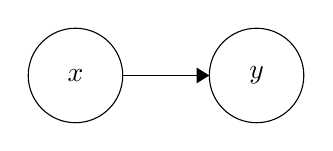
\begin{tikzpicture}[scale=0.2]
          \tikzstyle{every node}+=[inner sep=0pt]
          \draw [black] (16.5,-23.2) circle (3);
          \draw (16.5,-23.2) node {$x$};
          \draw [black] (28,-23.2) circle (3);
          \draw (28,-23.2) node {$y$};
          \draw [black] (19.5,-23.2) -- (25,-23.2);
          \fill [black] (25,-23.2) -- (24.2,-22.7) -- (24.2,-23.7);
     \end{tikzpicture}
\end{center}
The simplest way to build such a graph would be to scan every syntax tree searching for variables and then add edges accordingly. The inductive procedure could be implemented as follows
\begin{lstlisting}
interface Regex{
    void forEachVariable(Consumer<Variable> callback);
}
class Union implements Regex{
    Regex a; 
    Regex b;
    void forEachVariable(Consumer<Variable> callback){
        a.forEachVariable(callback);
        b.forEachVariable(callback);
    }
}

... the rest is done analogically...

class Variable implements Regex{
    void forEachVariable(Consumer<Variable> callback){
         callback.accept(this);
    }
}

class String implements Regex{
    java.lang.String str;
    void forEachVariable(Consumer<Variable> callback){
    }
}
\end{lstlisting}
The dependency graph is implemented using JGraphT library. It comes with a specialised data structure for directed acyclic graphs that guarantees acyclicity and throws exception whenever a newly added edge violates this property.
\begin{lstlisting}
DirectedAcyclicGraph<String, Object> dependencyOf =
    new DirectedAcyclicGraph<>(null, null, false);
\end{lstlisting}
The graph can be build by iterating all the definitions stored in \texttt{shared} map.
\begin{lstlisting}
for (Map.Entry<String, SolomonoffWeighted> def : shared.entrySet()) {
    String identifier = def.getKey();
    SolomonoffWeighted syntaxTree = def.getValue();
    syntaxTree.forEachVariable(var->{
        dependencyOf.add(
            var.identifier, // source vertex
            identifier, // target vertex
            new Object() // unique edge
        );
    });
}
\end{lstlisting}
The above code was simple but it requires to first build the syntax tree and then scan it. As a result every node of the tree is visited twice - first time during creation and second time during scanning. It also requires using the 
\texttt{forEachVariable} function. It's possible to make this procedure even simper and more efficient. The dependencies could be collected on the spot as the parsing progresses. Because multiple files are parsed in parallel
and \texttt{DirectedAcyclicGraph} is not thread-safe, an intermediate temporary storage for edges was necessary. We could first collect all of the edges into a list of pairs.
\begin{lstlisting}
List<Pair<String,String>> dependsOn;
\end{lstlisting}     
The problem with such approach is that certain edges might be duplicated. For instance consider the regular expression that uses $x$ twice
\begin{lstlisting}
x = 'a' | 'b'
y = 'a' (x 'b' x)*
\end{lstlisting}
This would lead to adding edge \texttt{Pair.of("y","x")} twice into \texttt{dependsOn}. To prevent this we use a set instead of list. The constructor of parser listener takes the following form
\begin{lstlisting}
Set<Pair<String,String>> dependsOn;
ConcurrentHashMap<String,SolomonoffWeighted> idToAST;
Set<Pair<String,String>> dependsOn;
SolomonoffWeightedParser(
         ConcurrentHashMap<String,SolomonoffWeighted> shared,
         Set<Pair<String,String>> dependsOn){
    this.idToAST = shared;
    this.dependsOn = dependsOn;
}
\end{lstlisting}
The set can be made thread-safe by using the concurrent implementation from Java standard library.
\begin{lstlisting}
ConcurrentHashMap.newKeySet()
\end{lstlisting}
The parser listener is a state-based device. When a certain rule of the formal grammar is fully parsed, several of the listener's callbacks are fired. For instance when the following rule \texttt{FuncDef} is recognized
\begin{lstlisting}
funcs :
    funcs exponential='!!'? ID '=' mealy_union  # FuncDef
    | 
;
\end{lstlisting} 
it will first fire \texttt{enterFuncDef}, then recursively all the events hiding under \texttt{mealy\_union} are executed and at the very end comes the \texttt{exitFuncDef}. If the expression contained a reference to some variable identifier at any point, then the event \texttt{exitMealyAtomicVarID} will be fired at some point during evaluation of \texttt{mealy\_union} callbacks. As a result the following code can be used to collect all dependencies into a set of pairs.
\begin{lstlisting}
String currentVariable;

@Override
public void enterFuncDef(FuncDefContext funcDefContext) {
    currentVariable = funcDefContext.ID().getText();
}
@Override
public void exitFuncDef(FuncDefContext funcDefContext) {
    SolomonoffWeighted def = stack.pop();
    idToAST.put(currentVariable, def);
}
@Override
public void exitMealyAtomicVarID(MealyAtomicVarIDContext ctx) {
    final String id = ctx.ID().getText();
    dependsOn.add(Pair.of(currentVariable,id));
    stack.push(new Variable(id));
}
\end{lstlisting}
When the parsing finishes, all of the collected dependencies need to be converted into edges of a directed graph:
\begin{lstlisting}
for (Pair<String, String> dependency : dependsOn) {
    dependencyOf.addEdge(
        dependency.right(), 
        dependency.left(), 
        new Object()
    );
}
\end{lstlisting}
If at any point a cyclic dependency is detected, the method \texttt{addEdge} will throw an exception and build system will exit prematurely.
This concludes the second phase of build procedure. 

The third and last phase is to compile all syntax trees is the correct order and parallelise it as much as possible. The compilation procedure presented before was a minimal prototype that could work with a single variable-free syntax tree.
like follows
\begin{lstlisting}
interface Regex{
     Regex substitute(HashMap<String,Regex> substitution);
}
class Union implements Regex{
     Regex a; 
     Regex b;
     Regex substitute(HashMap<String,Regex> substitution){
          return new Union(
              a.substitute(substitution),
              b.substitute(substitution)
          );
     }
}

... the rest is done analogically...

class Variable implements Regex{
     String identifier;
     Regex substitute(HashMap<String,Regex> substitution){
          return substitution.get(identifier);
     }
}

class String implements Regex{
     java.lang.String str;
     Regex substitute(HashMap<String,Regex> substitution){
          return this;
     }
}
\end{lstlisting}
 As a result all syntax trees would become variable-free. This comes at the cost of possibly exponential blow-up in size of certain trees. The major advantage is that now all trees can be compiled in parallel, although despite this, the compilation might in reality get worse than if we serially compiled trees with variables. That's because the overall number of nodes to be compiled could increase exponentially and the number of truly parallel threads (the number of cores in CPU) is usually small. Hence a better approach is needed. 
 
 The right solution is to compile all trees in parallel and block on variables that have not yet been processed.
 \begin{lstlisting}
 interface Regex{
      G compile(Function<String,Regex> blockingSubstitution);
 }
 class Union implements Regex{
      Regex a; 
      Regex b;
      G compile(Function<String,Regex> blockingSubstitution){
           return specs.union(
               a.compile(blockingSubstitution),
               b.compile(blockingSubstitution)
           );
      }
 }
 
 ... the rest is done analogically...
 
 class Variable implements Regex{
      String identifier;
      G compile(Function<String,Regex> blockingSubstitution){
           return blockingSubstitution.apply(identifier);
      }
 }
 
 class String implements Regex{
      java.lang.String str;
      G compile(Function<String,Regex> blockingSubstitution){
           return specs.fromStr(str);
      }
 }
\end{lstlisting}
The \texttt{blockingSubstitution} mimics the \texttt{HashMap.get} function but is more generalised. It allows us to provide lambda implementation 
that lookups a "lazy" map. Such a feature can be obtained by keeping a map of future promises. 
\begin{lstlisting}
ConcurrentHashMap<String, SolomonoffWeighted> shared;
ConcurrentHashMap<String,Future<G>> compiled;

... phase 1 and 2 ...

for(String variable : dependencyOf.vertexSet()){
	SolomonoffWeighted syntaxTree = shared.get(variable);
    compiled.put(id, pool.submit(() -> 
        syntaxTree.compile((referencedVar)->
            compiled.get(referencedVar).get() // may block
    );
}
\end{lstlisting}
The above snippet is simple but taking a closer look will reveal that its in fact incorrect. The \texttt{compiled.get(referencedVar)} might return \texttt{null} if
dependencies are not submitted before all their dependants. To prevent this we need to use topological order on directed acyclic graphs. The JGraphT provides a ready-made \texttt{TopologicalOrderIterator}. 

Every time we perform \texttt{pool.submit} the task is added to queue of tasks that will be picked up by some available thread in \texttt{ExecutorService}.By submitting those tasks in topological order we also guarantee optimal queue arrangement. The minimal number of threads will block on \texttt{get()} function as a result.
